\documentclass[spanish, 12pt, a4paper]{article}
\usepackage{graphicx}
\usepackage{hyperref}
\usepackage[spanish, mexico]{babel}
\usepackage[utf8]{inputenc}
\usepackage{xcolor}
\usepackage{listings}
\usepackage[margin=3cm]{geometry}

\usepackage{csquotes}
\usepackage[
  backend=biber,
  citestyle=alphabetic,
  ]{biblatex}
\addbibresource{refs.bib}

\definecolor{backcolor}{rgb}{0.95,0.95,0.92}
\lstset{
  basicstyle=\ttfamily\small,
  backgroundcolor=\color{backcolor},
  breaklines=true
}

\title{Notas Sueltas: Pro Git}

\begin{document}
\section{What is Git?}

\subsection{Snapshots, Not differences}

Los sistemas VCS usuales tienen un control de versiones
\emph{delta-based}. Guardan listas de cambios por archivo.

Git guarda snapshots de todos los archivos modificados y guarda
apuntadores a cada estado. Cada repositorio de git es una copia completa
y funcional del proyecto, no requiere dependencias externas y es todo
local.

Git hace checksums en cada commit, lo cual hace difícil o imposible
modificar sin que Git se de cuenta o perder información porque todo se
verifica y valida.

\subsection{The Three States}

Git tiene tres estados en los que puede estar un archivo en cualquier
momento dado:

\begin{itemize}
\item
  \textbf{Modified}: El archivo tiene modificaciones pero
  aún no se le ordena a Git incluir los cambios en el siguiente ``commit''
  o confirmación.
\item
  \textbf{Staged / Preparado}: El archivo fue modificado y marcado para
  que Git lo observe y guarde su versión actual en el siguiente commit.
\item
  \textbf{Commited / Confirmado}: Los cambios al archivo ya fueron
  observados y confirmados. Se guarda el estado actual del archivo en la
  base de datos de Git.
\end{itemize}

Adicionalmente hay archivos que pueden estar dentro del directorio, en
disco, y no existir dentro de la base de datos Git. Los tres estados
anteriores solo aplican para archivos \emph{rastreados} o
\emph{tracked}. Los archivos \emph{no-rastreados} o \emph{untracked}
siguen dentro del alcance de búsqueda de Git, y éste aún los puede ver,
pero tiene instrucciones de no rastrear modificiaciones.

Similarmente, hay tres secciones o ``espacios'' en cada proyecto de Git:

\begin{enumerate}
\item
  Working Directory.
\item
  Staging Area.
\item
  Git Repository.
\end{enumerate}

\emph{Working Directory} es el directorio ``fisico'', local en tu
máquina en donde estás trabajando. Es como cualquier otra carpeta, pero
tiene la particularidad de que hay una instancia de Git observándola. El
\emph{Working Directory} es el \underline{checkout} de una versión
particular del proyecto. Los archivos fueron descomprimidos de la base
de datos de Git, y puestos en el disco para poder ser modificados como
cualquier otro archivo.

\emph{Staging Area} se puede pensar como el lugar físico a donde se
mandan los archivos que están marcados como listos para ser confirmados
(commited). En realidad es un archivo, pero la abstracción de lugar es
más útil.

\emph{Git repository} es donde vive la base de datos de Git, y todos los
metadatos asociados. Aqui se guardan las diferentes versiones
comprimidas de cada commit hecho, asi como apuntadores y metadatos de
documentación. El archivo .git es el que contiene toda esta información,
y es el que obtiene uno al clonar un repositorio.

Un archivo particular se considera \emph{commited} (confirmado) si fue
modificado, añadido al \emph{staging area}, y se hizo un \emph{commit}
(confirmación). Los cambios que se le hicieron a ese archivo ahora están
grabados en git. Un archivo se considera \emph{staged} (preparado) si se
modifició y se añadió al \emph{staging area}. Un archivo se considera
\emph{modified} (modificado) si sufrió cambios desde la última versión
que conoce Git, pero aún no se añade al \emph{staging area}. Los
archivos \emph{modified} que no sean añadidos al \emph{staging area}
antes de efectuar un \emph{commit} no serán rastreados en ese
\emph{commit}, y sus cambios no se guardarán.


\subsection{Basic Git Workflow}

\begin{enumerate}
\item
  Modifica archivos locales en disco.
\item
  Se elige qué archivos se desea rastrear (\emph{track}) añadiéndolos al
  \emph{staging area}. Son estos y solo estos los archivos que serán
  parte de la siguente confirmación.
\item
  Se lleva a cabo una \emph{confirmación}, en la que se toman un
  snapshot del estado actual del \emph{staging area} y se guarda
  permanentemente en el repositorio Git, junto con datos de
  identificación y mensajes de confirmación.
\end{enumerate}

\subsection{Command Line Interface}

Para obtener ayuda sobre el comando

\begin{lstlisting}
$ git add -h
usage: git add [<options>] [--] <pathspec>...

    -n, --dry-run         dry run
    -v, --verbose         be verbose

    -i, --interactive     interactive picking
    -p, --patch           select hunks interactively
    -e, --edit            edit current diff and apply
    -f, --force           allow adding otherwise ignored files
    -u, --update          update tracked files
    --renormalize         renormalize EOL of tracked files (implies -u)
    -N, --intent-to-add   record only the fact that the path will be added later
    -A, --all             add changes from all tracked and untracked files
    --ignore-removal      ignore paths removed in the working tree (same as --no-all)
    --refresh             don't add, only refresh the index
    --ignore-errors       just skip files which cannot be added because of errors
    --ignore-missing      check if - even missing - files are ignored in dry run
\end{lstlisting}

\section{Git Basics}

\subsection{Getting a Git Repository}

Usualmente uno obtiene un repositorio de Git en dos maneras:

\begin{enumerate}
\item
  Tomas cualquier carpeta local en tu disco, y la conviertes en un
  repositorio con \texttt{git\ init}, o bien
\item
  \emph{Clonas} un repositorio de Git existente de algún otro lugar.
\end{enumerate}

Para crear un repositorio nuevo desde una carpeta local, basta con
navegar hasta la carpeta deseada a través de la terminal de comandos, y
ejecutar el comando \texttt{git\ init} que creará un repositorio nuevo
con todo lo necesario para usar Git, y rastrear cambios en los archivos
de ese directorio. El comando \texttt{init} crea un ``esqueleto de
git''. En este punto, ningun archivo está siendo rastreado, todos
aparecen como \emph{untracked}. Si deseas empezar a rastrear cambios,
debes cambiar el estatus de los archivos de \emph{untracked} a
\emph{tracked} a través del commando \texttt{git\ add}. Cabe mencionar
que los archivos nuevos, es decir los originales en un directorio antes
de correr \texttt{git\ init}, o aquellos creados o añadidos después de
haber creado el repositorio, siempre aparecerán por primera vez como
\emph{untracked}, hasta que se le señale a Git que se deben rastrear.

\begin{quote}
Notas: El comando \texttt{git add} tiene dos funciones: Cambia el
estatus de un archivo de \emph{untracked} a \emph{tracked}, y además
añade archivos \emph{modified} al \emph{staging area} para prepararlos
para un \emph{commit}.

\texttt{add} recibe como argumento nombres de archivos, o patrones
\emph{glob}.
\end{quote}

Tradicionalmente una vez que se han rastreado los archivos de interés se
hace un ``primer commit''.

\begin{lstlisting}
$ git commit -m "Primer commit"
\end{lstlisting}

El modificador \texttt{-m} es corto para \texttt{message}, y quiere
decir que le mensaje de confirmación viene en seguida rodeado de
comillas, como en el ejemplo de arriba. Si no se usa el modificador
(flag) \texttt{-m}, Git abrirá el editor de texto default de la
terminal, por ejemplo Vim, y estarás atrapado y confundido.

Si deseas copiar un repositorio existente, por ejemplo, para contribuir
a algún proyecto o con tu equipo, entonces se crea un nuevo repositorio
con \texttt{git\ clone}. El comando \texttt{clone} recibe de argumento
un URL a algún repositorio remoto. Por ejemplo, el comando a
continuación clona el repositorio donde está alojado el libro Pro Git,
de Scott Chacon, con base en el cual se hicieron estas notas.

\begin{lstlisting}
$ git clone https://github.com/progit/progit2
\end{lstlisting}

El comando clone crea una nueva carpeta en el directorio actual donde
residirá el repositorio \texttt{.git} junto con los archivos en el que
corresponde a la versión que clonaste. En automático el nombre de la
carpeta que se va a crear es el nombre del repositorio, en este caso
``progit2'', pero también es posible especificar un nombre distinto. Por
ejemplo, si queremos que la nueva carpeta se llame ``libro-git'',
pasamos ese nombre como argumento adicional, es decir:

\begin{lstlisting}
$ git clone https://github.com/progit/progit2 libro-git
\end{lstlisting}

\subsection{Recording Changes}

Una vez que se tiene un repositorio de Git y archivos rastreados, se
puede empezar a usar todo el potencial de Git.

\begin{figure}
  \centering
  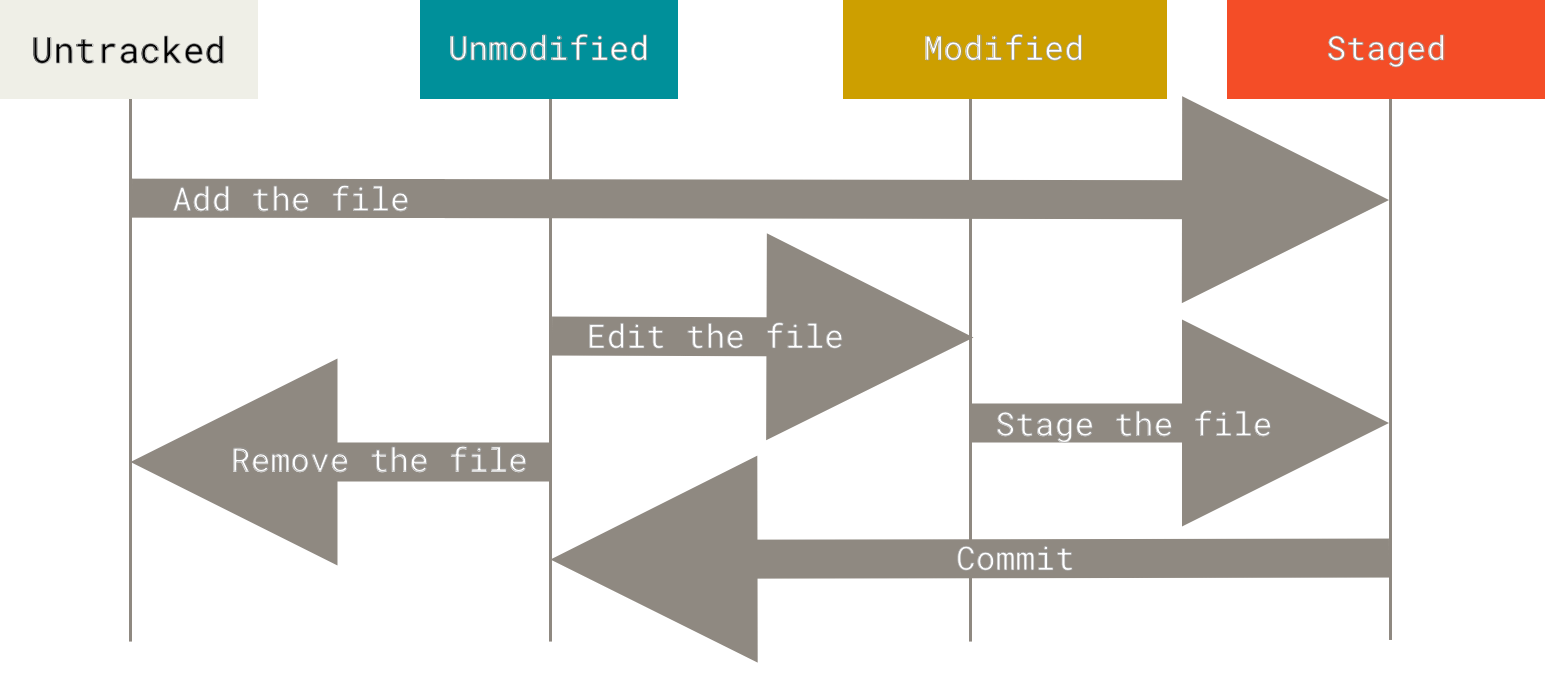
\includegraphics[width=\textwidth]{figs/lifecycle.png}
  \caption{Ciclo de vida de un archivo en un Git Repo.}
  \label{fig:lifecycle}
\end{figure}

Como habíamos dicho, un archivo puede estar en uno de cuatro estados en cualquier momento dado: \textit{untracked}, \textit{unmodified}, \textit{modified}, \textit{staged}, como lo muestra la figura \ref{fig:lifecycle}.

Para checar en qué punto del ciclo se encuentran los archivos existe el comando \texttt{git status}.
Por ejemplo, al correrlo cuando se ha iniciado un nuevo repo o no se han hecho cambios desde el último \textit{commit}, se ve asi:

\begin{lstlisting}
$ git status
On branch master
Your branch is up-to-date with 'origin/master'.
nothing to commit, working directory clean
\end{lstlisting}

Con la frase ``working directory clean'' quiere decir que no hay cambios para el siguiente \textit{commit}, ya sea porque no se han rastreado los archivos o porque los archivos rastreados no han sido modificados desde el último \textit{commit}.
Si se añaden archivos nuevos desde el último commit al correr \texttt{git status} saldrá un mensaje similar:
\begin{lstlisting}
Untracked files:
  (use "git add <file>..." to include in what will be committed)

        ejemplo.txt
\end{lstlisting}
con lo cual vemos que el archivo es reconocido por Git, pero que los cambios que se le hagan o su estado actual no serán rastreados por git.

Una vez que se empieza a rastrear un archivo y se hace un primer \textit{commit} con el y se empiece a modificar, la siguiente vez que se corra \texttt{git status}, mostrará algo como lo siguiente: 
\begin{lstlisting}
On branch master
  Changes not staged for commit:
    (use "git add <file>..." to update what will be committed)
    (use "git checkout -- <file>..." to discard changes in working directory)
  
          modified:   ejemplo.txt
\end{lstlisting} 
Eso no quiere decir que el archivo (en este caso \texttt{ejemplo.txt}) dejó de ser rastreado por Git y que se perdió el historial de cambios, sino que Git reconoce los cambios hechos al archivo y ahora está esperando a que se añada al \textit{staging area} mediante \texttt{git add}, ya que Git deja al usuario decidir qué cambios se toman en cuenta para un commit dado, en vez de asumir que todos los cambios entre un \textit{commit} y el siguiente son todos relacionados con lo mismo.

Cubiertos los básicos, hay un flag (opción) que se puede pasar al comando \texttt{git status} para hacerlo más corto y facil de entender: el flag \texttt{-s} que es corto para \texttt{--short}.
\begin{lstlisting}
$ git status -s
  M  ejemplo.txt
  A  anadido.txt
  ?? otro.txt
\end{lstlisting}

Ahora en vez de listar archivos como \textit{staged}, \textit{modified}, etc\dots Git muestra una lista corta de los archivos de interés con una letra mayúscula a su izquierda.
Esa letra a la izquierda se llama \underline{código de estatus}.

\begin{table}[h]
  \centering
  \begin{tabular}{|c|l|}
    \hline
    Código de Estatus & Significado \\
    \hline \hline
      & Sin modificar \\
    \hline
    \textbf{M} & Modificado \\
    \hline
    \textbf{A} & Añadido \\
    \hline
    \textbf{D} & Eliminado (deleted) \\
    \hline
    \textbf{R} & Renombrado \\
    \hline
    \textbf{C} & Copiado \\
    \hline
    \textbf{U} & Actualizado (updated)\\
    \hline
    \textbf{??} & Untracked (sin rastrear) \\
    \hline 
  \end{tabular}
  \caption{Guía de códigos de estatus para \texttt{git status -s}}
\end{table}

\subsection{Ignoring Files}
Muchas veces hay archivos temporales que se crean al correr código en los cuales no estamos interesados.
Para evitar que Git esté listándolos siempre que se corra \texttt{status} o añadirlos por error, se puede crear una lista de archivos que no nos interesa rastrear y preferimos que Git ignore por completo.
Esto se hace a través de un \texttt{.gitignore}.

Un \texttt{.gitignore} es un archivo que le dice a Git que archivos no estamos interesados en rastrear.
Por ejemplo, puede que no estemos interesados en archivos \texttt{.log}, o en archivos \texttt{.aux} que se crean con la compilación de archivos \TeX.
En vez de listarlos por nombre, podemos utilizar \underline{patrones}.
Para esto se utilizan patrones Glob, que son como expresiones regulares (regex) simplificadas.
El ejemplo mas simple es el siguiente:
\begin{lstlisting}
# Git ignore para proyecto x 
*.log
*.aux
Build/
\end{lstlisting}

La primera linea empieza con un \#, y se toma como un comentario.
Usualmente es util para aclarar el propósito del \texttt{.gitignore} u otras cosas.
El patrón \texttt{*.log} quiere decir ``ignora todos los archivos que terminen con \texttt{.log}''.
Ese mismo patron se puede usar con la extensión de archivo que sea, \texttt{.log} no tiene nada de especial.
Análogamente el patrón \texttt{Build/} indica que no se debe rastrear nada dentro de la carpeta \texttt{Build} ni de sus subdirectorios.
Afortunadamente, no hace falta tener esto en cuenta la mayoría del tiempo.
GitHub mantiene una librería de \texttt{.gitignore}s estándar para una gran variedad de lenguajes de programación y proyectos, la cual está disponible en \url{https://github.com/github/gitignore}.

\subsection{Viewing Staged and Unstaged Changes}
Para revisar y comparar cambios con la versión anterior de un archivo el comando \texttt{status} no es muy útil.
El comando para esto es \texttt{git diff}.
Cuando se corre el comando \texttt{diff} sin argumentos Git mostrará una comparación de los archivos que están en el área de trabajo (\textit{working directory}) y la versión que está en el \textit{Staging Area}, es decir que está lista para ser confirmada.
Si se quiere comparar los cambios que ya fueron mandados al \textit{Staging Area}, y que serán efectuados al siguiente \textit{commit}, se corre con los argumentos \texttt{git diff --staged}.
Con el arugmento \texttt{staged} se compara el \textit{commit} más reciente con los cambios hechos a un archivo desde ese \textit{commit}.

Ahora bien, correr \texttt{git diff} directamente en la terminal abre el editor Vim en modo de lectura, lo cual no siempre es lo más cómodo porque Vim no es precisamente intuitivo.
En la práctica es más facil dejar que esto lo haga una de las interfaces gráficas de Git.
En la mayoría de los casos vienen integradas con tu editor o IDE, y si todo eso falla puedes utilizar el comando \texttt{git difftool --tool} para ver que visualizadores tienes disponibles, o simplemente \texttt{git difftool} para lanzar la herramienta default\footnote{Cuidado. Este es uno de los comandos que te pueden dejar atrapado en Vim. Si nunca has usado Vim es mejor usar otra interfaz gráfica.}.

\subsection{Committing Your Changes}
Una vez que hayas terminado los cambios que deseabas hacer y los añadiste al \textit{Staging Area}, es momento de guardar el estado actual de los archivos mediante un \textit{commit}.
Para esto, tenemos el comando con un nombre adecuado, \texttt{git commit}.
Una vez más, este comando tiene flags opcionales.
En este caso la importante es \texttt{-m}, corto para \texttt{--message}.
En caso de que no se pase esta opción, Git lanzará el editor por defecto de la terminal, en muchos casos Vim.
Para evitar quedar atrapado en Vim, puedes usar
\begin{lstlisting}
$ git commit -m "Mensaje de commit"
\end{lstlisting}
para poner un mensaje de confirmación o \textit{commit message} sin necesidad de abrir un editor de texto.
Tradicionalmente el \textit{commit message} se utiliza para listar los cambios hechos desde el último \textit{commit} en caso de que sea necesario revertir a ese estado por alguna razón.

Un ejemplo de el output de \texttt{git commit -m}, sacado de Pro Git.
\begin{lstlisting}
$ git commit -m "Story 182: fix benchmarks for speed"
  [master 463dc4f] Story 182: fix benchmarks for speed
   2 files changed, 2 insertions(+)
   create mode 100644 README
\end{lstlisting}

En el texto de salida del comando vemos algunas cosas interesantes.
Por ejemplo vemos el nombre del \textit{branch} o rama al que se confirmaron tus cambios (en este caso \texttt{master})\footnote{más sobre ramás adelante}, y un código alfanumérico llamado checksum, en este caso \texttt{463dc4f}, y un resumen corto de los cambios, inserciones y eliminaciones.

Dado que la mayoría del tiempo se quieren agregar todos los archivos modificados al staging area sería deseable poder brincar el comando \texttt{git add .} y confirmar todos los cambios en un solo comando.
Para eso existe el flag \texttt{-a}, el cual equivale a añadir todos los cambios al \textit{Staging Area} y luego confirmarlos con \texttt{commit}.
Los flags \texttt{-a} y \texttt{-m} se pueden usar juntos, pero poneindo \texttt{-m} al final (puesto que la sintaxis usual de interfaces de command line espera el argumento de un flag inmediatamente después de que se utilice este flag).
Por ejemplo:
\begin{lstlisting}
$ git commit -a -m "Fixes"
\end{lstlisting}

\section{Removing Files}
Para quitar archivos del repositorio de Git hay que sacarlos de los archivos rastreados.
Para eso existe el comando \texttt{git rm}.
Mucho cuidado, \texttt{rm} no solo remueve el archivo de la base de datos de Git, también lo elimina en tu \textit{Working Directory}!
Para quitarlo de los archivos rastreados sin eliminarlo del directorio local se utiliza la opción \texttt{--cached}.
Cabe mencionar que este comando acepta no solo nombres de archivos, sino patrones Glob como se mencionó antes.

\subsection{Viewing the Commit History}
El punto entero de tener un sistema de control de versiones es poder registrar cambios graduales, por eso se tiene el sistema de commits.
En caso de ser necesario, se puede navegar a puntos anteriores en el tiempo, y revertir a esos cambios.
También se puede experimentar en el proyecto sin temor a dañar algo y que sea irreversible.

Para revisar el historial de cambios y confirmaciones existe el comando \texttt{git log}.
Por ejemplo, al correrlo dará un resultado como este:
\begin{lstlisting}
$ git log
  commit ca82a6dff817ec66f44342007202690a93763949
  Author: Scott Chacon <schacon@gee-mail.com>
  Date:   Mon Mar 17 21:52:11 2008 -0700
  
      Change version number
  
  commit 085bb3bcb608e1e8451d4b2432f8ecbe6306e7e7
  Author: Scott Chacon <schacon@gee-mail.com>
  Date:   Sat Mar 15 16:40:33 2008 -0700

      Remove unnecessary test

  commit a11bef06a3f659402fe7563abf99ad00de2209e6
  Author: Scott Chacon <schacon@gee-mail.com>
  Date:   Sat Mar 15 10:31:28 2008 -0700

      Initial commit
\end{lstlisting}

Al correr \texttt{git log} sin argumentos se obtiene una lista de los commits del repo en orden cronológico inverso.
Cada listado tiene la información relevante del commit: el checksum que sirve como identificación única, nombre y correo electrónico del autor, la fecha y hora de confirmación, y el mensaje que se dió.

El comando \texttt{log} tiene una variedad de opciones.
Por ejemplo, la opción \texttt{-n} muestra los $n$ commits más recientes.
La opción \texttt{-p}, corto para \texttt{--patch}, muestra los cambios hechos por cada commit.
Equivale a correr \texttt{diff} sobre cada commit individualmente.
La opción \texttt{--stat} da estadísticas rápidas sobre cada commit como el número de líneas modificadas.

Si el resultado aparece demasiado extenso hay una opción para hacerlo más legible: \texttt{--pretty}.
La opción \texttt{--pretty} funciona como un diccionario key-value.
Es decir, se utiliza con otras opciones, por ejemplo \texttt{oneline}, \texttt{short}, \texttt{full}, \texttt{fuller}.
Si se necesita aún más flexibilidad el comando acepta un objeto tipo \textit{format}, en el que se le puede especificar un \textit{string format} para acomodar los datos que se crean convenientes en la forma deseada.
Puesto que no es muy común no incluyo más detalles. Se pueden encontrar mejores referencias en \cite[pág.~88]{chacon-2009}, o simplemente corriendo \texttt{man git log}.

Una buena opción para un log corto es \texttt{git log --oneline --decorate}, que da por ejemplo:
\begin{lstlisting}
$ git log --oneline --decorate               
a3eb382 (HEAD -> master) Viewing commit history
ca82a6d Change version number
17c4c59 Remove unnecessary test
6cdc27e Initial commit
\end{lstlisting}
que solo muestra el número identificador abreviado y el mensaje de confirmación.

Cuando se está trabajando con diferentes ramas el comando \texttt{git log --graph --oneline --decorate} muestra un arbol con las ramas de desarrollo y su interacción entre ellas.
Hablaremos con más detalle de ramas más adelante.

Vale la pena mencionar que Git hace una distinción entre \textit{author} y \textit{committer}.
Es decir, el autor es quien hizo los cambios, el confirmador (\textit{committer}) es simplemente quien los confirmó.

El comando log tiene aún más opciones y funciones, las cuales no tiene sentido revisar ahora.

\subsection{Undoing things}
Quizás una de las más grandes ventajas de usar un VCS es poder revertir cambios, pero hay que tener en cuenta que no todo se puede, y si no se tiene cuidado se pueden perder cosas de manera permanente.
La mayoría de los siguientes comandos y cómo se hace lo que se describe a continuación viene en pequeñas instrucciones o pistas cuando se corre \texttt{git status} sin argumentos.

Por ejemplo, si se hizo un commit antes de tiempo, se puede usar el comando \texttt{commit} una vez más, pero con la opción \texttt{--amend}.
Esto incorpora los cambios sin duplicar una confirmación.
También es util para modificar el mensaje de confirmación por si se quiere añadir más información.

Otro error comun es añadir dos archivos al \textit{Staging Area} cuando alguno de los dos no estaba listo, o simplemente porque se quiere confirmar los cambios por separado.
El comando \texttt{git reset HEAD <archivo>} sacan el archivo seleccionado del \textit{Staging Area} pero conservan las modificaciones.

Ahora bien, ¿cómo revierto los cambios no deseados a un archivo?
Para des-modificar un archivo y regresarlo al estado en el que estaba en el último commit, se usa \texttt{git checkout -- <archivo>} para des-modificar \texttt{archivo}.
Hay que tener mucho cuidado al usar este comando, porque reemplaza el archivo en el \textit{Working Directory} completamente por otra vesión de el. No hay forma de deshacer estos cambios (ni con ctrl-z).

Más adelante discutimos mejores prácticas para guardar temporalmente cambios y otras técnicas.

\subsection{Working with Remotes}
Introducimos el concepto de un \textit{Remote}.
Un \textit{remote} es una versión de tu Git Repo alojada en algún otro lugar, como el internet.
Gracias a los \textit{remotes} es que podemos colaborar en proyectos.
Para recuperar cambios o para subir los propios usamos los comandos \texttt{pull}, \texttt{fetch} y \texttt{push} que dicutimos más adelante.

Para listar los \textit{remotes} que tiene un repo podemos usar el comando \texttt{git remote} sin argumentos.
Si creaste un nuevo repo desde cero, \texttt{remote} no dará ningún resultado, porque aún no has configurado ningún \textit{remote} para el repo actual.
Si lo clonaste de algún lugar en internet el comando debería listar por lo menos un remote: \texttt{origin}, que es el nombre por defecto que recibe el \textit{remote} original de donde fue clonado el repositorio local.
El comando sin argumentos solo da los nombres con los cuales tiene guardados los \textit{remotes}, lo cual no siempre es lo más útil.
Corriendo \texttt{git remote -v} obtenemos una lista no solo de los \textit{remotes} disponibles sino también el \textsc{url} al que nos estamos comunicando para subir y bajar cambios\footnote{Un \textit{remote} no necesariamente está fuera de tu propia computadora, podría ser un repo local, y todo funcionaría igual.}.

Como decíamos, clonar un repo automáticamente añade el origen como un \textit{remote}, y lo nombra \texttt{origin} apropiadamente.
Para añadir \textit{remote}s nuevos se usa el comando \texttt{git remote add <shortname> <url>}.
Por ejemplo, el \textsc{url} que va entre corchetes es el \textsc{url} de la página de GitHub en donde estará alojado el repo.
Una vez que se tiene configurado un \textit{remote} es fácil jalar o empujar cambios.
El \texttt{shortname} que le asignaste al crear un \textit{remote} es el nombre con el que será conocido desde ese momento, y con el cual te referirás para jalar o empujar cambios.
Es decir, actúa como un alias para todo el \textsc{url}.

\subsubsection{Pulling}
Para jalar los cambios que están en el \textit{remote}, existe el comando \texttt{git fetch <remote>}, que se traduce como ``ir a buscar'', o ``traer''.
El \texttt{remote} entre corchetes es el nombre corto que se le asignó a el \textit{remote} del cual se quiere hacer \textit{fetch} al momento de configurarlo.
Este comando baja la versión más reciente del repo disponible en el \textit{remote}, pero \underline{no combina (\textit{merge}) los cambios.}
\texttt{fetch} solo obtiene la versión más reciente y la almacena en una nueva rama\footnote{más sobre ramas más adelante}, pero no incorpora los cambios a tu versión de los archivos.
El estado de los archivos en tu \textit{Working Directory} no se ve afectado por \texttt{fetch}, y para incorporar los cambios se tendría que hacer una unión (\textit{merge}) entre la rama actual y la que se creó, lo cual discutiremos a detalle en la sección sobre ramas.
Afortunadamente, el comando \texttt{git pull <remote> <branch>} ahorra el proceso de unir ramas, y además de bajar los cambios más recientes del \textit{remote}, los combina automáticamente con el estado actual de los archivos en el \textit{Working Directory}.
Lo realmente interesante de Git está en lo que está escrito arriba: Git puede combinar cambios automáticamente y en la mayoría de los casos, sin ninguna clase de ayuda.
Hablaremos más tarde de qué se hace cuando Git encuentra cambios conflictivos entre el estado de un archivo en el \textit{Working Directory} y la versión en el \textit{remote}. 

\subsubsection{Pushing}
Cuando deseas publicar tu versión del repo y el estado actual de los archivos rastreados, puedes usar el comando \texttt{git push <remote> <branch>} para \textit{empujar} los cambios a el \texttt{remote} que se da como argumento, a la rama que se especifica también entre corchetes.

Un detalle importante es que para hacer \textit{push} a un \textit{remote}, tu versión local debe estar al día con la versión más reciente en el \textit{remote}.
Si el \textit{remote} tiene cambios más recientes a los que están en tu \textit{Working Directory}, Git te pedirá que bajes los cambios del remoto y actualices tu versión a la que bajaste.
Hasta entonces se puede hacer \textit{push}.

Cabe mencionar que no siempre se tiene permiso de hacer \textit{push} a cualquier repositorio, se necesita que el dueño te de permiso.

Cuando se tienen diferentes \textit{origin}s a los que se empuja y jala regularmente, a veces es util pedir ayuda para recordar qué nombre corto está asociado a qué \textsc{url}, entre otras cosas.
El comando \texttt{git remote show <remote>} da más información acerca del \textit{remote} asociado al nombre corto que se da como argumento.
Dependiendo del caso de uso el comando puede dar mucha información.
Por ahora no damos más detalles al respecto.

También es posible cambiar el nombre corto de un \textit{remote} después de haberlo configurado.
Esto se hace con \texttt{git remote rename <oldname> <newname>}.

Análogamente, es fácil remover remotos, como cuando ya no se utilizan más.
Esto se hace mediante \texttt{git remote remove <remote>}.

\subsubsection{Tagging}
Otra habilidad de Git es etiquetar (\textit{tag}) \textit{commit}s específicos; lo cual es muy util cuando hubo cambios importantes o ese commit particular está asociado a una versión importante o algo del estilo.

Listar los \textit{tags} existentes es fácil, se hace con \texttt{git tag}.
Si no se ha etiquetado ningún \textit{commit}, el comando no regresará nada.
Cabe mencionar que el orden en el que se listan los resultados es alfabético, no cronológico.

Un uso interesante es revisar una serie específica de versiones, por ejemplo, si se corre \texttt{git tag -l "v1.8.5*"} en el repositorio donde está alojado el código fuente de Git, podemos ver la serie de versiones 1.8.5.$x$.
\begin{lstlisting}
$ git tag -l "v1.8.5*"
  v1.8.5
  v1.8.5-rc0
  v1.8.5-rc1
  v1.8.5-rc2
  v1.8.5-rc3
  v1.8.5.1
  v1.8.5.2
  v1.8.5.3
  v1.8.5.4
  v1.8.5.5
\end{lstlisting}
En este ejemplo, el \texttt{*} que se usa en el string después del switch \texttt{-l} (corto para \texttt{--list}) es un ejemplo de una expresión regular, y quiere decir ``cualquier caracter''.

Git permite dos tipos de \textit{tags}: \textit{lightweight} y \textit{annotated}.
El tipo \textit{lightweight} es solo una referencia a un punto particular del historial de \textit{commits}.
Un \textit{tag} del tipo \textit{annotated} se guarda como su propio \textit{commit}, y tiene toda la información que contendría uno, como la fecha, autor, etc\dots
Por ejemplo, se puede crear una etiqueta anotada como
\begin{lstlisting}
$ git tag -a v1.0 -m "Version 1!"
\end{lstlisting}
El swith \texttt{-a} es corto para \texttt{--annotated}.

Para crear una etiqueta ligera, se usa el comando \texttt{tag} sin las opciones \texttt{-a} ni \texttt{-m}.
Por ejemplo 
\begin{lstlisting}
$ git tag v1.0
\end{lstlisting}

Ahora puedes revisar la información del \textit{commit} que fue etiquetado.
Eso se hace con \texttt{git show <tag>}.

También es posible etiquetar \textit{commit}s que se hicieron en el pasado.
Eso se hace con \texttt{git tag <tag> <hash>} en donde \texttt{hash} es el código de identificación corto que está asociado al checksum de un \textit{commit} particular.
Este \texttt{hash} sale por ejemplo al correr \texttt{git log} con sus posibles opciones.

Por default Git no comparte los \textit{tags} hechos localmente, se tiene que empujar mediante \texttt{push} como si fueran ramas independientes.
Aún más facil que eso, se puede correr \texttt{git push <remote> --tags} para subir todos los \textit{tags} al \textit{remote} sin necesidad de hacerlo uno a uno.
Cabe mencionar que el comando anterior empuja ambos tipos de \textit{tags}: anotadas y ligeras.

Para eliminar \textit{tags} existe el flag \texttt{-d}, corto para \texttt{--delete}.
Por ejemplo, si queremos eliminar el \textit{tag} de ejemplo que hicimos arriba, corremos
\begin{lstlisting}
$ git tag -d v1.0
\end{lstlisting}
Sin embargo, esto no va a eliminar las etiquetas del \textit{remote} al que fueron subidas.
Si se quiere eliminar también del remote, se usa
\begin{lstlisting}
$ git push <remote> --delete <tagname>
\end{lstlisting}

% ToDo: Checking out tags.
% Creo que vale la pena explicar checkout antes de esto.

Nota: Se pueden crear aliases para evitar escribir comandos largos con argumentos complejos.

\section{Git Branching}
El workflow de ramas (\textit{branches}) permite bifurcar el estado de los archivos en el \textit{Working Directory} para hacer modificaciones, sin arruinar el estado de la rama principal.
Es usual crear ramas para desarrollar nuevas funciones, o incluso para hacer pruebas sin temor de arruinar un proyecto funcional.
También es muy usual en un workflow de equipo tener diferentes ramas para cada integrante del equipo, o para sub-equipos.

El comando para crear nuevas ramas es 
\begin{lstlisting}
$ git branch <branchname>
\end{lstlisting}

El crear nuevas ramas implica solamente crear un nuevo apuntador, que empieza apuntando al la rama en el cual se creó, en el mismo punto en el que se creó.

\begin{figure}[h]
  \centering
  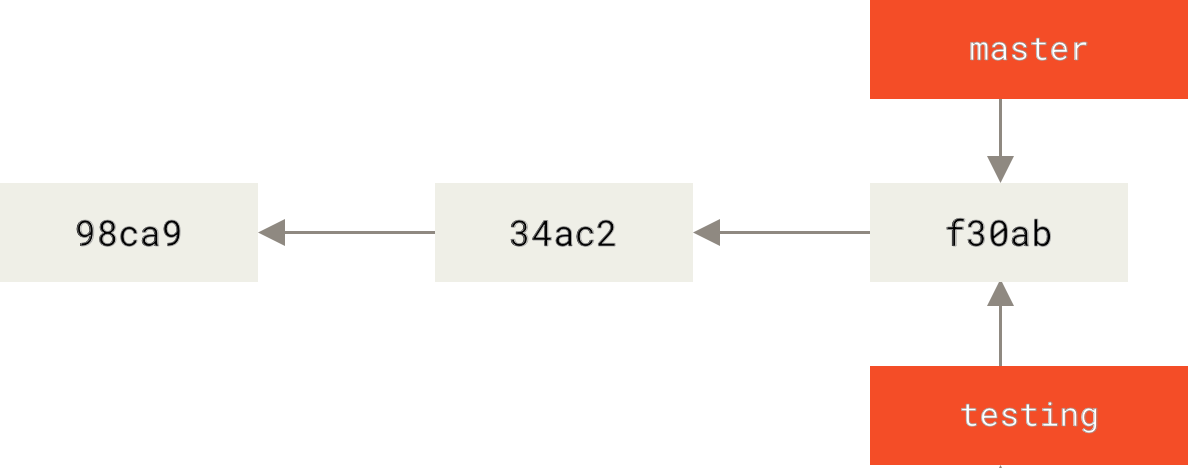
\includegraphics[width=\textwidth]{figs/two-branches.png}
  \caption{Creación de una nueva rama.}
  \label{fig:two-branches}
\end{figure}

En la figura \ref{fig:two-branches} se muestra un ejemplo de lo que pasa cuando se crea una nueva rama.
Las cajas grises con códigos hash unidas por flechas constituyen la rama original, usualmente llamada \textit{master}.
Cada caja gris representa un \textit{commit}, representada por el código hash que la identifica.
La caja amarilla apuntando al \textit{commit} \texttt{f30ab} representa al apuntador que viene con cada rama, en ese caso el apuntador original que identifica a la rama, por eso tiene el nombre \texttt{master}.
En el momento en el que se crea una nueva rama aparece el nuevo apuntador (caja naranja), en este caso llamada \texttt{testing}.
Esa nueva caja llevará el nombre de la nueva rama recién creada, y es la que se encarga de apuntar a los cambios que se hicieron \underline{mientras se trabajaba en esa rama}.
En el momento en que se haga un nuevo \textit{commit} estando en \texttt{testing}, el apuntador naranja avanzará, dejando atrás a \texttt{master}.
A partir de ese punto se pueden combinar (\textit{merge}) las ramas \texttt{master} y \texttt{testing} para ponerlas al día, o bien, regresar el estado de \texttt{testing} a como estaba en \texttt{master}.

El apuntador especial \texttt{HEAD} indica a Git en qué punto se está trabajando en un momento dado.
Es decir, apunta a la rama y el punto sobre ella sobre el cual se escribirá al hacer un nuevo \textit{commit}.

\begin{figure}[h]
  \centering
  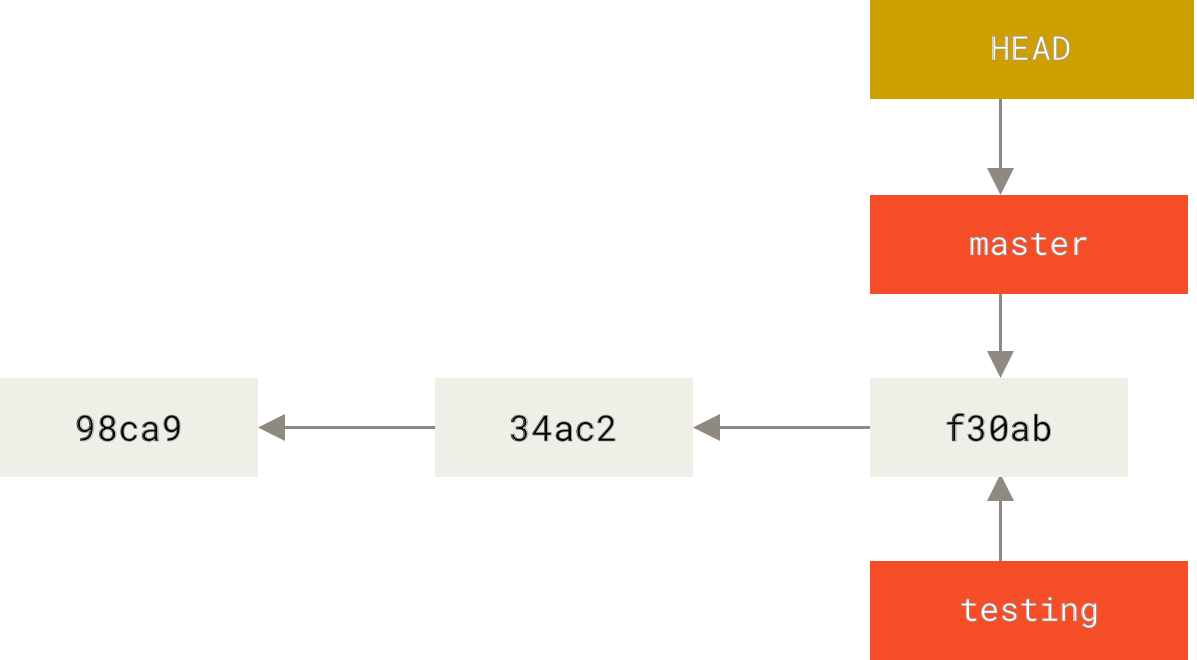
\includegraphics[width=\textwidth]{figs/head-to-master.png}
  \caption{\texttt{HEAD} apuntando a \texttt{master}}
\end{figure}

Para cambiar de rama, es decir mover el apuntador \texttt{HEAD} para apuntar a \texttt{testing} y empezar a hacer \textit{commit} ahi, usamos el comando
\begin{lstlisting}
$ git checkout <branch>
\end{lstlisting}

A la rama activa se le dice la rama \textit{checked-out}.
Esto claro tiene que ver con que el comando para activar y crear ramas es \texttt{git checkout}, pero \texttt{checkout} hace más que eso.

Si ahora hacemos un nuevo \textit{commit} después de haber cambiado a \texttt{testing} pasará lo siguiente: 

\begin{figure}[h]
  \centering
  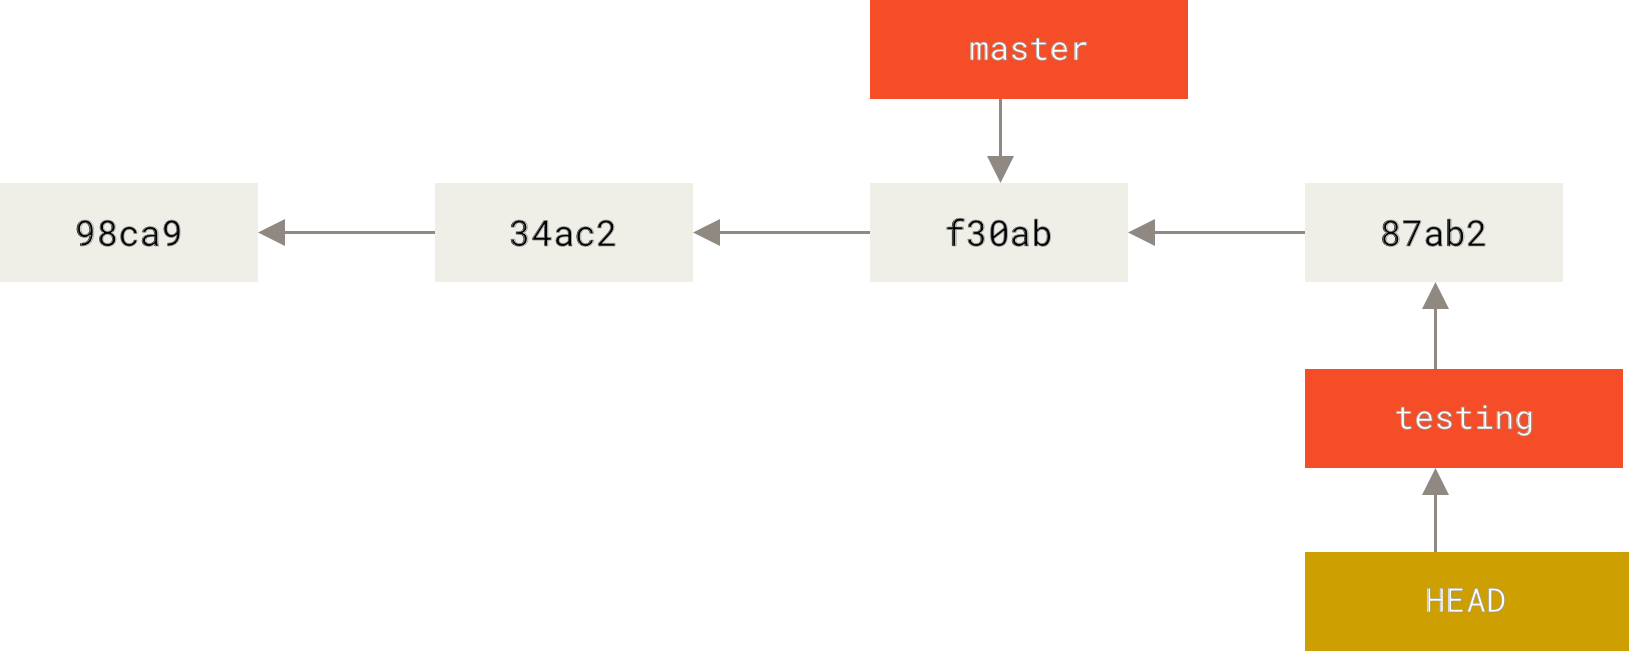
\includegraphics[width=\textwidth]{figs/advance-testing.png}
  \caption{\texttt{HEAD} avanzó dejando atrás \texttt{master}.}
\end{figure}

Si corremos el comando
\begin{lstlisting}
$ git checkout master
\end{lstlisting}
en este momento, \texttt{HEAD} los archivos del \textit{Working Directory} volverán al estado en el que estaban en ese momento, y además se moverá \texttt{HEAD} de vuelta a ese punto.
Es decir, si hacemos un nuevo \textit{commit} en este punto, ahora habrá una bifurcación entre \texttt{master} y \texttt{testing}.

\begin{figure}[h]
  \centering
  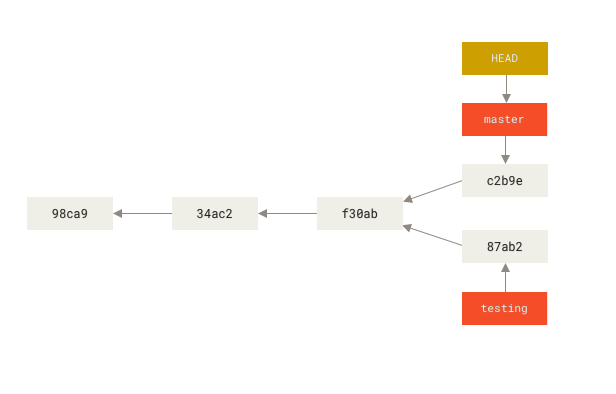
\includegraphics[width=\textwidth]{figs/advance-master.png}
  \caption{Bifurcación entre \texttt{master} y \texttt{testing}.}
  \label{fig:bifurcacion}
\end{figure}

Como muestra la figura \ref{fig:bifurcacion}, al hacer nuevos \textit{commits} se hace avanzar \texttt{HEAD}.
Ambas ramas convergen en \texttt{f30ab} porque son el ancestro que tienen en común.
Para visualizar estos movimientos se puede usar \texttt{git log --oneline --decorate --graph --all}.

Para crear una rama nueva y moverse a ella en un solo comando, se utiliza \texttt{git checkout} con la opción \texttt{-b}, corto para \texttt{--branch}.
Por ejemplo
\begin{lstlisting}
$ git checkout testing
\end{lstlisting}
crea una nueva rama llamada \texttt{testing}, y además mueve \texttt{HEAD} a ella para que el siguiente \textit{commit} se haga sobre la nueva rama.

\subsection{Basic Branching and Merging}
El procedimiento básico para unir (\textit{merge}) dos ramas es moverse, o ``activar'' (\textit{checkout}) la rama hacia la cual se va a unir, y correr el comando \texttt{git merge <branch>}.
Hay diferentes tipos de \textit{merge}s que pueden ocurrir.
Cuando la rama que se unió estába directamente adelante, sin cambios divergentes, Git lleva a cabo una unión \textit{fast-forward} (avance rápido).
Es decir, Git simplemente mueve el apuntador \texttt{HEAD} hacia adelante.

Si después de unir dos ramas ya no necesitas la que fue unida, la puedes eliminar fácilmente con el comando \texttt{branch} y la opción \texttt{-d}, corto para \texttt{--delete} 
\begin{lstlisting}
$ git branch -d <branch>
\end{lstlisting}

Cuando intentas unir dos ramas con cambios divergentes, o a la que se intenta unir no es ancestro directo de la que se une, Git no puede hacer una unión \textit{fast-forward}.
En esos casos, Git tiene que hacer una unión entre tres commits (\textit{three-way merge}), que podemos pensar como nodos sobre las ramas.
Sin embargo, como los cambios en ambas ramas no conflictúan entre sí, Git aún puede hacer una unión simple; es decir, una que no requiere intervención del usuario.
Cuando esto sucede, se dice que no hay conflictos.
En este caso particular, la unión se hace entre los dos nodos usuales más un tercer nodo que es su ancestro común más cercano.

Al unir dos ramas, Git combina los contenidos de manera automática (si puede), y automáticamente crea un nuevo \textit{commit}.

\subsubsection{Basic Merge Conflicts}
Hay ocasiones en las que Git no puede hacer uniones simples y necesita consultar con un usuario cuales cambios mantener.
Estos conflictos se dan cuando se intentan fusionar (unir) dos ramas que tienen cambios que no son compatibles entre si.
Por ejemplo, cuando se modifica un archivo de dos maneras distintas en el mismo lugar con respecto a el ancestro en común más cercano.

Un ejemplo de cuando no se puede hacer una unión limpia:
\begin{lstlisting}
$ git merge iss53
Auto-merging index.html
CONFLICT (content): Merge conflict in index.html
Automatic merge failed; fix conflicts and then commit the result.
\end{lstlisting}

Cuando sucede un conflicto, Git pausa el proceso de unión que culmina con un \textit{commit} y espera a que el usuario resuelva los conflictos.
Si corremos \texttt{git status} después de un conflicto, podemos ver en qué archivos se dió el conflicto para empezar a solucionarlo
\begin{lstlisting}
$git status
On branch master
You have unmerged paths.
  (fix conflicts and run "git commit")

Unmerged paths:
  (use "git add <file>..." to mark resolution)

    both modified:      index.html

no changes added to commit (use "git add" and/or "git commit -a")
\end{lstlisting}

En el ejemplo anterior el conflicto se dió en el archivo \texttt{index.html}.
Cuando ocurre un conflicto Git modifica los archivos y les añade marcadores para ayudar a resolver el conflicto.
Estos marcadores están para que se pueda abrir manualmente el archivo, y decidir qué cambios se quedan y cuales se van.
Abriendo el archivo con conflicto, se vería algo como esto:
\begin{lstlisting}
<<<<<<< HEAD:archivo.txt
Contenido en HEAD. Es decir, rama local hacia la cual se hace la union
=======
Contenido en branch, rama que esta siendo unida a HEAD
>>>>>>> branchname:archivo.txt
\end{lstlisting}

Entre los corchetes de apertura \texttt{<<<<<<<} y el separador \texttt{=======} están los cambios que están en donde actualmente se encuentra \texttt{HEAD}.
Es decir, los cambios en la rama que está activada actualmente, hacia la cual se quiere unir.
En el encabezado se aclara en qué rama está, y el archivo que tuvo conflictos.
En la parte desde el separador hasta los corchetes de cerradura \texttt{>>>>>>>} están los cambios \textit{incoming}.
Es decir, los que están en la rama que se está tratando de unir.

Algunos editores de texto y IDEs están configurados para reconocer estos bloques generados automáticamente por Git, y dan ayuda visual poniendolos en fondos de colores, o dando botones de ayuda para aceptar cambios \textit{incoming}, mantener el estado actual, o incluso mantener ambos.
Si tu editor o IDE no tiene esta funcionalidad, puedes usar las herramientas visuales que vienen con Git, corriendo \texttt{git mergetool}.

Para resolver un conflicto se eligen los cambios a mantener (o se borran ambos), y se quitan los marcadores generados por Git.
Una vez que se decidió qué cambios mantener y se añade el archivo resuelto (sin marcadores) al \textit{Staging Area}, Git entenderá que el conflicto fue resuelto.
Si se corre \texttt{git status} en este punto Git pedirá confirmación de que se resolvió exitosamente el conflicto.
Para finalizar la unión se confirman todos los cambios con \texttt{git commit}.
Nótese que ahora no escribimos un mensaje de confirmación, Git lo añade automáticamente con la información más importante para señalizar que hubo una unión y resolución de conflicto.

\subsubsection{Branch Management}
El comando \texttt{git branch} al usarse sin argumentos va a listar todas las ramas del repo, y marca la activa con un \texttt{*} al lado izquierdo de su nombre.
Para mostrar el \textit{commit} más reciente en cada rama, se puede usar \texttt{git branch -v}.

A veces es util ver si las ramas tienen cambios incorporados a la rama actual, o si aún no se han unido.
Para esto existen las opciones \texttt{--merged} y \texttt{--no-merged} que actúan como filtro.
Por ejemplo al correr
\begin{lstlisting}
$ git branch --merged
  mergedbranch 
* master
\end{lstlisting}
vemos que la rama \texttt{mergedbranch} ya fué unida a \texttt{master}.
Como ya está unida, es seguro eliminarla con \texttt{git branch -d mergedbranch} sin ningún peligro.
Sin embargo, si intentamos eliminar una rama que no ha sido unida, digamos \texttt{unmerged-b}, Git nos dará un error y pedirá confirmación.
\begin{lstlisting}
$ git branch -d unmerged-b
error: The branch 'unmerged-b' is not fully merged.
If you are sure you want to delete it, run 'git branch -D unmerged-b'.
\end{lstlisting}

Como muestra el mensaje de ayuda del comando anterior, se puede sobreescribir el mecanismo de Git diseñado para no perder cambios usando el switch \texttt{-D} (en mayúscula).
Esto solo se hace si estás consciente de que se perderán todos los cambios en esa rama.
Por ejemplo, si era una rama \textit{throwaway} en la que se hizo un experimento. 

\subsection{Branching Workflows}
En esta subsección revisamos algunos de los \textit{workflows} más comunes que se usan para trabajar con Git y ramas.
Esto es en realidad más descriptivo que normativo, pero es útil para estructurar proyectos grandes.
En especial porque estos \textit{workflows} están diseñados para evitar conflictos a la hora de las uniones, y tener tantas uniones simples como sea posible.

\subsubsection{Long-Running Branches}
La estructura de desarrollo de ramas \textit{long-running} se basa en tener un número pequeño de ramas principales que siempre están abiertas, dedicadas a las diferentes etapas del desarrollo, las cuales se unen entre si de manera regular.

Una estrategia común es tener dos ramas principales: \textit{master} y \textit{development} (los nombres no son importantes).
En \texttt{master} se tiene el código en su estado más pulido, mientras que en \texttt{development} se hacen los cambios importantes que solo se unen a \texttt{master} una vez que están terminados, probados, etc\dots
Es usual agregar una rama o serie de ramas más dedicadas a resolver problemas particulares.
Estas ramas se unen a \texttt{development} una vez que se resolvió aquello para lo cual fueron creadas, y se eliminan poco después.
Este tipo de ramas se conocen como \textit{topic branches}, o ramas de tema.

Es útil pensar en las ramas estructuradas de esta manera como almacenes en los que se guarda código en función de su madurez.

% ToDo:
% Remote branches

\subsection{Rebasing}
Como el nombre sugiere, consiste en cambiar de base una versión particular.
Es decir, es como hacer los cambios que se efectuaron a través de una rama, como si se hubieran hecho empezando desde otro punto de la rama o de otra rama por completo.
\begin{lstlisting}
$ git rebase master
\end{lstlisting}

La operación funciona encontrando al ancestro común de las dos ramas que se están uniendo, y aplicando lo cambios gradualmente.
Una vez que se hace un \textit{rebase}, se puede hacer un \textit{merge} simple del tipo \textit{fast-forward} hasta la punta de la rama.
Todo eso gracias a que ahora la punta de la rama y el \textit{commit} al que se hizo el \textit{rebase} tienen una ancestría en común, una ancestría lineal.
Ya no hay ningún conflicto de versiones.

Vale la pena hacer notar que el producto final no tiene nada de diferente a hacer un \textit{merge}.
La única ventaja notable es que hace que la historia de \textit{commits}, los logs, esté más limpio y claro.

Hay rebases más complejos, pero francamente no entendí del todo, y valdrá la pena revisarlo con más calma.

\section{Distributed workflows}


\end{document}